\documentclass[10pt,a4paper]{article}
\usepackage[utf8]{inputenc}
\usepackage[margin=1in]{geometry}
\thispagestyle{empty}

\usepackage[spanish]{babel}

\usepackage{amsmath}
\usepackage{amsfonts}
\usepackage{amssymb}

\usepackage{parskip}

\usepackage{listings}
\usepackage{xcolor}

\usepackage{enumerate}

\usepackage{hyperref}

\usepackage{float}
\usepackage{wrapfig}

\usepackage{graphicx}
\restylefloat{figure}

\usepackage[font=small,labelfont=bf]{caption}
\usepackage{subcaption}

\usepackage{cancel}

\usepackage{multicol}
\setlength{\columnsep}{22pt}

\usepackage{colortbl}
\usepackage{verbatim}

\DeclareMathOperator*{\argmin}{arg\,\min}
\DeclareMathOperator*{\argmax}{arg\,\max}

\author{Cristian Escudero\\\small{Con agradecimientos a Marcos Yedro}}
\title{Resumen Final\\Inteligencia Computacional}
\begin{document}

\maketitle
%%%%%%%%%%%%%%%%%%%%%%%%%%%%%%%%%%%%%%%%%%%%%%%%%%%%%%%%%%%%%%%%%%%%%%%%%%%%%%%%%%%%%%%
\part{Inteligencia Colectiva}
\setcounter{section}{0}

\section{Resolver problemas mediante búsqueda}

\subsection{Nociones Básicas}

\subsubsection{Definición de agente}

Un \textbf{agente} es cualquier cosa capaz de percibir\footnote{La idea de \textbf{percepeción} indica que el agente puede recibir entradas en cualquier instante.} su \textbf{medioambiente} con la ayuda de \textbf{sensores} y actuar en ese medio utilizando \textbf{actuadores} (\textit{reacciona al estímulo ejecutando una acción}).

En general, un agente tomará una decisión en un momento dado dependiendo de la \textbf{secuencia completa de percepciones} -\textit{historial completo de lo que ha recibido}- hasta ese instante.

El comportamiento del agente viene dado por la \textbf{función del agente} que transforma una percepción dada en una acción. Esta última se implementará mediante un \textbf{programa del agente}. La diferencia es que la \textit{función} es una descripción matemática abstracta y el \textit{programa} es la implementación completa.

\subsubsection{Diferencia entre agente y programa/objeto}

El \textbf{agente} se diferencia de un \textbf{programa} \textit{per se} en lo que respecta a la capacidad de afectar el entorno. El agente cambia el problema, el programa no, ya que este último solo recibe una entrada y devuelve una salida, no ejecuta ninguna acción al respecto. Además, el programa solo se ejecuta una vez, el agente se mantiene continuamente activo.

La diferencia entre un \textbf{agente} y un \textbf{objeto} (o \textit{clase}), es que el primero puede actuar autónomamente (puede no responder como yo deseo) en base al conocimiento acumulado.

\subsubsection{Definición de agente racional}

Un \textbf{agente racional} es aquel que hace lo \textbf{correcto}; es decir, en cada posible secuencia de percepciones, debe emprender aquella acción que supuestamente maximice su \textit{medida de rendimiento}\footnote{Las \textbf{medidas de rendimiento} incluyen los criterios que determinan el éxito en el comportamiento del agente. Se prefieren criterios objetivos que estén apuntados a lo que se quiera para el entorno.}, basándose en las evidencias aportadas por la secuencia de percepciones y en el conocimiento que mantenga almacenado.

Una \textbf{acción} es una operación que causa una transición entre estados del mundo.

\subsubsection{Clasificación}

\begin{itemize}
\item \textbf{Agentes reactivos.} Basan sus acciones en una aplicación directa desde los estados a las acciones. No funcionan bien en entornos en los que esta aplicación sea demasiado grande para almacenarla y que tarde mucho en aprenderla. Se clasifican a su vez en:
\begin{itemize}
\item \textbf{simples}, que no utilizan \textit{historial} para tomar decisiones; ó \item \textbf{basados en modelos}, que mantienen un \textit{estado interno} que depende del \textit{historial} para tomar decisiones.
\end{itemize} 
\item \textbf{Agentes basados en objetivos.} Pueden tener éxito considerando las acciones futuras y lo deseable de sus resultados.
\begin{itemize}
\item \textbf{Agente resolvedor de problemas.} Está basado en el anterior; deciden qué hacer para encontrar \textit{secuencias de acciones} que conduzcan a los \textbf{estados deseables}.
\end{itemize}
\end{itemize}

Además están los \textbf{agentes basados en utilidad}, que elige decisiones en base a un sistema de prioridad.

Por último, los \textbf{sistemas multiagentes} contienen varios tipos de agentes, que pueden competir o colaborar para lograr un objetivo.

\subsection{Agentes resolvedores de problemas}

Básicamente, el diseño simple del agente es: \textit{formular, buscar} y \textit{ejecutar}.

El primer paso para solucionar un problema es la \textbf{formulación de un objetivo}, basado en la situación actual y la medida de rendimiento del agente. Un \textbf{objetivo} es un conjunto de estados del mundo (estados en los cuales el objetivo se encuentra satisfecho). Requiero una forma de medir si llegue o no a mi objetivo.

Dado un objetivo, la \textbf{formulación del problema} es el proceso de decidir que acciones y estados hay que considerar. Un agente con distintas opciones inmediatas de valores desconocidos puede decidir qué hacer, examinando las diferentes secuencias posibles de acciones que le conduzcan a estados de valores conocidos, y entonces escoger la mejor secuencia. Este proceso de hallar esta secuencia se denomina \textbf{búsqueda}.

\makebox[\textwidth]{
\fbox{\textit{Entrada}: Problema}$\rightarrow$\fbox{\textbf{Algoritmo de búsqueda}}$\rightarrow$\fbox{\textit{Salida:} Solución}
}

En la última fase, la de \textbf{ejecución} se proceden a ejecutar las acciones que recomienda la solución.

\subsection{Problemas y soluciones bien definidos}

Un problema puede \textbf{definirse} mediante cinco componentes:
\begin{enumerate}
\item \textbf{Estado inicial} en el que comienza el agente.
\item \textbf{Conjunto de acciones disponibles}. Pueden incluir información sobre requisitos y consecuentes.
\item \textbf{Espacio de estados del problema,} que es el conjunto de todos los estados alcanzables desde el estado inicial por cualquier secuencia de acciones.
\item \textbf{Test objetivo,} el cuál determina si un estado es el \textit{estado objetivo}.
\item \textbf{Función de evaluación del costo del camino,} que asigna un costo numérico a cada secuencia de acción.
\end{enumerate}

El \textbf{proceso de búsqueda} puede ser pensado como la construcción de un \textbf{árbol de búsqueda} el cual está superpuesto al \textit{espacio de estados}, donde la raíz corresponde al \textit{estado inicial}. El \textbf{estado a expandir} está determinado por la \textbf{estrategia de búsqueda}.

\subsubsection{Árbol de Búsqueda}

Una posible estructura para representar los nodos del árbol es la siguiente:
\begin{enumerate}
\item \texttt{Estado:} del \textit{espacio de estados} que corresponde al nodo.
\item \texttt{Nodo Padre:} el nodo que lo ha generado.
\item \texttt{Acción:} que se aplicará al padre para generar el nodo.
\item \texttt{Costo del Camino:} desde el estado inicial al nodo.
\item \texttt{Profundidad:} que es el número de pasos a lo largo del camino desde el estado inicial.
\end{enumerate}

\underline{Nota:} un \textit{estado} no es lo mismo que un \textit{nodo}. El primero es una representación de la configuración física, y el segundo es una estructura de datos que forma parte del árbol de búsqueda.

\subsection{Medir el rendimiento de la resolución del problema}

Las \textbf{estrategias de búsquedas} (que determinan el próximo nodo a expandir) se consideran a partir de los siguientes criterios:
\begin{itemize}
\item \textbf{Completitud:} \textit{¿encuentra solución si ésta existe}?
\item \textbf{Complejidad:} se clasifica en \textbf{\textit{temporal}} (\textit{¿cuánto tiempo tarda}?) y \textbf{\textit{espacial}} (\textit{¿cuánta memoria ocupa}?). Es medida en función de:
\begin{itemize}
\item Máximo factor de ramificación del árbol ($b$).
\item Profundidad de la solución más barata ($d$).
\item Profundidad máxima del espacio de estado ($m$).
\end{itemize}
\item \textbf{Optimalidad.} \textit{¿encuentra la solución de mejor calidad entre las disponibles}?
\end{itemize}

A la vez se clasifican en:
\begin{itemize}
\item \textbf{Búsqueda no informada.} No tienen información adicional acerca de los estados más allá de los que proporciona la definición del problema. No conoce que tan cerca está del objetivo. Dentro de esta categoría, tenemos los siguientes métodos de búsqueda:
\begin{enumerate}
\item \textbf{Horizontal:} construye un árbol que va creciendo a lo ancho. Es \textbf{completa} (al menos encuentra una solución), y además la solución puede ser \textbf{óptima} (si el costo es uno en cada etapa). Tiene mucho costo \textbf{espacial} (guarda todo el árbol en memoria) y \textbf{temporal}. Es una buena alternativa si esto último no es problema.
\item \textbf{Profundidad:} construye el árbol yendo hacia abajo. Si la solución no la encuentra, retrocede y desciende por otra rama. No es \textbf{completa} (falla en espacios infinitos y con búcles de estados repetidos) ni da la solución \textbf{óptima}. Es muy \textbf{rápido} y requiere \textbf{poco espacio} (necesita almacenar sólo un camino desde la raíz a un nodo hoja, junto con los nodos hermanos restantes no expandidos para cada nodo del camino).
\item \textbf{Profundidad Iterativa:} es como el anterior, pero iterativamente fija profundidades incrementales. Esta alternativa permite que el algoritmo sea \textbf{completo} y \textbf{óptimo} (si el costo es uno en cada etapa). Es \textbf{rápido} y \textbf{liviano}.
\item \textbf{Costo Uniforme:} va expandiendo los nodos y calculan los costos, eligiendo siempre los nodos con menor costo. El problema es como asignar costos a los caminos. Es \textbf{completo} y \textbf{óptimo}. El \textbf{tiempo} y el \textbf{espacio} que use puede ser alto, dependiendo esto mucho de la función que utilice para calcular los costos.
\item \textbf{Bidireccional:} expande los nodos desde el \textit{estado inicial} con una búsqueda hacia delante y desde el \textit{estado final} con una búsqueda hacia atrás (requiere necesidad de poder calcularse nodos predecesores). Requiere definir los algoritmos de búsqueda usados en ambos sentidos. Es \textbf{completa} y \textbf{óptima} (si la búsqueda utilizada es la horizontal). Es muy costosa en \textbf{tiempo} y \textbf{espacio} (requiero dos árboles de búsqueda).
\end{enumerate}
\item \textbf{Búsqueda informada.} Saben si un estado no-objetivo es ``\textit{más prometedor}'' que otro. Lo que se hace es aplicar una \textit{función de evaluación} (que suele ser una \textit{estimación}) en el nodo, para ir midiendo el avance. En estos métodos se expande siempre el ``\textit{mejor}'' nodo (\textbf{\textit{método de búsqueda primero el mejor}}). Existen dos enfoques:
\begin{enumerate}
\item \textbf{Avara:} utiliza solamente la heurística (\textit{cuánto me falta para llegar}) para tomar las decisiones. Siempre expando el nodo que se estima más cercano al objetivo. No es \textbf{completa} (pueden existir búcles) y no es \textbf{óptima}. Es bastante costosa en \textbf{tiempo} y \textbf{espacio}.
\item \textbf{A$^*$:} combina la heurística con el \textit{costo} (desde el nodo inicial) para tomar las decisiones. Es \textbf{óptima} y \textbf{completa}, si se aplica la restricción de que el mínimo costo estimado al objetivo no se sobre-estime. La elección de una buena función heurística es necesaria para disminuir la complejidad tanto en \textbf{tiempo} como en \textbf{espacio}. Está dentro de los mejores métodos de búsqueda.
\end{enumerate}
\end{itemize}

\underline{Nota:} hay que tratar que los nodos de estados repetidos no se repitan al generar los hijos, para evitar búcles infinitos.

\section{Planificación}

La \textbf{planificación} es el proceso de \textit{búsqueda y articulación} de una \textbf{secuencia de acciones} que permitan alcanzar un objetivo.

\subsection{Lenguaje de los problemas de planificación}

Plantear el problema de búsqueda usualmente exige demasiadas \textbf{acciones} y \textbf{estados} para analizar.

Algunas de las características que requiere cumplir el problema para ser resuelto con planificación:
\begin{itemize}
\item Representación \textbf{explícita} del objetivo, para evitar ser desbordado por acciones irrelevantes al problema. Se ha de encontrar una \textbf{función heurística}\footnote{Se puede definir \textbf{heurística} como un arte, técnica o procedimiento práctico o informal, para resolver problemas.} adecuada (para que los algoritmos de búsqueda sean eficientes). El tomar decisiones obvias o importantes en forma temprana permite reducir el \textbf{factor de ramificación}, disminuyendo la necesidad de \textbf{\textit{back-tracking}}.
\item \textbf{Descomposición} del problema en sub-problemas (pero frecuentemente no es posible), aunque después necesita trabajo adicional para combinar los \textbf{sub-planes} resultantes.
\item Suposición de \textbf{independencia} de objetivos. Si hay algun conflicto, voy a tener mecanismos para resolverlo.
\item Entornos: \textbf{completamente observables} (el agente conoce a todo momento todas las variables del entorno), \textbf{determiníticos} (el próximo estado del medio solo depende del actual y de lo que haga el agente), \textbf{estáticos} (los cambios los producen los agentes) y \textbf{discretos} (en tiempos, acciones, efectos y objetos).
\end{itemize}

La \textbf{representación de los problemas} de planificación (\textit{acciones}, \textit{estados} y \textit{objetivos}) debe hacer posible que los algoritmos de planificación se aprovechen de la estructura lógica del problema. El lenguaje de representación básico de los planificadores clásicos se llama \texttt{STRIPS}, y la idea de este es que sea suficientemente \textbf{expresivo} (para representar una gran gama de problemas) a la vez que \textbf{restrictivo} (para permitir algoritmos operativos y eficientes). Algunas de las características de \texttt{STRIPS} son:
\begin{itemize}
\item \textbf{Representación de estados.} Utiliza representaciones completas de los estados. Posee un conjunto de literales \textit{lógicas de primer orden} (\textit{sin dependencias funcionales}) \textbf{positivas} (\textit{sin negaciones}) y \textbf{simples}. Se asume \textbf{hipótesis de mundo cerrado} (\textit{todas las condiciones no mencionadas son tomadas como falsas}) y \textbf{espacio de estados finito}.
\item \textbf{Representación de objetivos.} Solo se tiene un test para verificar el objetivo y una función heurística.
\item \textbf{Representación de acciones.} Consisten en funciones que generan descripciones de estados sucesores. Una \textbf{acción} se representa a través de: \textit{precondiciones} (\textit{literales que tienen que ser verdadero}) y \textit{efectos} (\textit{agreguen/saquen literales}).
\end{itemize}

La planificación va creando entonces un \textbf{plan} y se van incorporando las acciones en cualquier lugar que sean necesarias. No hay necesariamente una conexión entre el \textbf{orden} en que se \textit{genera} el plan y el orden en que se \textit{ejecuta}.

\subsection{Operadores \texttt{STRIPS}}

Un \textbf{operador} (instancia de una regla) \texttt{STRIPS} se define mediante \textbf{esquemas de representación}. La descripción \textbf{explícita} de los \textit{operadores} permite proceder con un enfoque \textbf{hacia atrás} (\textit{regresión}), debido a que estos tienen suficiente información para \textbf{regresar} desde la descripción parcial de un \textbf{estado} hasta la descripción parcial del \textbf{estado precedente}.

El enfoque de \textbf{regresión} es preferible, ya que usualmente, la descripción del objetivo tiene pocos elementos, para los cuales hay pocos operadores que pueden producirlos. Además, se consideran sólo las acciones \textbf{relevantes}.

\subsection{Planificador de Orden Parcial}

Las búsquedas anteriores son \textbf{totalmente ordenadas}: solo exploran secuencias estrictamente lineales de acciones conectadas directamente al inico o al objetivo. Esto evita sacar provecho de la \textbf{descomposición} del problema.

En este enfoque se \textit{flexibiliza} el \textit{orden} en que se \textbf{construye} el plan, tomando las decisiones usando un sistema de prioridades.

Características del \textbf{orden parcial} (POP):
\begin{itemize}
\item El planificador trabaja sobre \textbf{sub-metas} en forma independiente una de otra.
\item No se preocupa del orden de los pasos durante la búsqueda.
\item Estrategia: \textbf{mínimo compromiso}, en la que se aplazan las opciones hasta un punto en el que se pueda seguir progresando en la búsqueda.
\item Pueden aparecer dos acciones en un plan sin identificar orden entre ellas.
\end{itemize}

A la solución dada por un POP hay que \textbf{linealizarla}. Es decir, ordenar los pasos. Por ende, puede haber muchas linealizaciones de una misma secuencia de acciones (por ejemplo, \textit{poner media izquierda y luego derecha, o al revés}) que den a lugar varios posibles planes de \textbf{orden total}.

Para que un plan sea una \textbf{solución}, debe ser:
\begin{itemize}
\item \textbf{Completo.} Un plan es \textit{completo} $\iff$ se han alcanzado todas las
\textbf{precondiciones}. 
\subitem + Una \textit{precondición} se ha alcanzado $\iff$ es el efecto de un paso anterior y no puede ser removida por otro paso.
\item \textbf{Consistente.} Para esto, se requiere que:
\subitem + No haya ciclos en las restricciones ordenadas.
\subitem + No haya conflictos con los vínculos causales.
\end{itemize}


%%%%%%%%%%%%%%%%%%%%%%%%%%%%%%%%%%%%%%%%%%%%%%%%%%%%%%%%%%%%%%%%%%%%%%%%%%%%%%%%%%%%%%%

\section{Computación Evolutiva}

La evolución es un proceso de \textbf{optimización}, donde el objetivo es mejorar la habilidad de los individuos de sobrevivir. La computación evolutiva (EC) es la emulación del proceso de \textbf{selección natural} en el procedimiento de búsqueda. En la naturaleza, los organismos poseen ciertas características que influyen sus habilidades de supervivencia y reproducción. Estas características están representadas por una larga cadena de información contenida en los \textbf{cromosomas} del organismo. Luego de la \textbf{cruza}, los cromosomas de los descendientes consisten de una combinación de la información de los cromosomas de los padres. Con suerte, el resultado obtenido es aquel que contiene la mejor parte de los cromosomas de ambos padres. El proceso de selección natural se asegura que los organismos que mejor se ``\textit{adapten}'' al entorno sean los que más posibilidades tengan de reproducirse, cuyos hijos estarán similarmente o incluso mejores adaptados.

Ocasionalmente, los cromosomas de un organismo son sujetos a \textbf{mutaciones} que pueden causar cambios en las características de dicho individuo. Estos cambios pueden tener una connotación negativa en la habilidad de supervivencia o reproducción del individuo, pero por otro lado, puede que esa mutación realmente mejore la adaptación del mismo, llevando de esa forma mayores probabilidades de supervivencia y producción de descendientes. Sin las mutaciones, la población tiende a converger a un estado homogéneo donde los individuos rararamente varían unos con otros.

La evolución vía la selección natural que elige individuos de la población aleatoriamente puede ser visto como una búsqueda a través del espacio de todos los valores de cromosomas posibles. En ese sentido, un \textbf{algoritmo evolutivo} (\textit{evolutive algorithm}, EA) es una búsqueda aleatoria por una solución óptima a un problema dado. El proceso de búsqueda evolutivo está influenciado por las siguientes componentes principales:
\begin{itemize}
\item una codificación de la solución al problema en forma de cromosoma;
\item una función que evalúa la capacidad de adaptación del individuo;
\item una inicialización de la población inicial;
\item operadores de selección natural; y 
\item operadores de reproducción.
\end{itemize}

Los EAs han sido aplicados a una gran amplia cantidad de áreas, incluyendo:
\begin{itemize}
\item planificación, como por ejemplo, optimización de rutas y calendarización;
\item diseño, como por ejemplo, el diseño de filtros y arquitecturas neuronales; y
\item minería de datos.
\end{itemize}

\subsection{Algoritmos genéticos}

Los \textbf{algoritmos genéticos} (GAs) son la clase más popular de EA, los cuales modelan la \textbf{evolución genética}. Las características de los individuos son entonces expresadas usando \textbf{genotipos}. Son utilizados frecuentemente en problemas de optimización.

\subsection{La evolución como un algoritmo}

\begin{enumerate}
\item[] {\color{darkgray} // Se comienza inicializando la población al azar.}
\item \texttt{Inicializar (\textit{población})}
\item[] {\color{darkgray} // Se decodifica el \textbf{genotipo} en \textbf{fenotipo} y evalúa el \textit{fitness} de c/individuo.}
\item \texttt{\textit{mejor\_fitness} = Evaluar (\textit{población})}
\item[] {\color{darkgray} // Entramos en el búcle de \textbf{optimización/búsqueda}.}
\item \texttt{\textbf{Mientras} (\textit{mejor\_fitness} $<$ \textit{fitness\_requerido})}
\begin{enumerate}[3.1]
\item[] {\color{darkgray} // Seleccionamos los padres de la nueva generación.}
\item \texttt{\textit{selección} = Seleccionar(\textit{población})}
\item[] {\color{darkgray} // Efectuamos las cruzas y las mutaciones.}
\item \texttt{\textit{población} = CruzarYMutar(\textit{selección})}
\item[] {\color{darkgray} // Finalmente, la \textit{población} nace y es evaluada.}
\item \texttt{\textit{mejor\_fitness} = Evaluar(\textit{población})}
\end{enumerate}
\item \texttt{FinMientras}
\end{enumerate}

\subsection{Elementos de un algoritmo evolutivo}

\begin{itemize}
\item \textbf{Representación de los individuos.} Determinar la traducción \textbf{fenotipo} $\leftrightarrow$ \textbf{genotipo}. El primer aspecto a resolver es el de codificar el problema en un diccionario finito.
\item \textbf{Función de \textit{fitness}.} Se debe poder medir que tan buena es cada solución en relación a las demás. Tiene las siguientes características generales:
\begin{itemize}
\item \textbf{Monoticidad.} Cuanto mejor la solución, más grande el número.
\item \textbf{Precisión.} Depedende de la cantidad de \texttt{bits} utilizados por los cromosomas.
\item \textbf{Suavidad Regulable.} Algún parámetro que permita graduar la suavidad, según el problema.
\item \textbf{Penalización de Complejidad.} Además de lograr la solución óptima, se desea que sea simple.
\end{itemize}
\item \textbf{Mecanismos de selección.} Elegir a los padres siguiendo probabilidades, como en la naturaleza. Se debe dar la posibilidad incluso de que los \textit{peores} individuos sean padres.
\item \textbf{Operadores de variación y reproducción.} los operadores básicos son cruzas y mutaciones, y hay varias formas de aplicarlos. A partir de los operadores podemos reproducir y obtener una nueva población.
\end{itemize}

\subsection{Diseño de una solución mediante algoritmos evolutivos}

\subsubsection{Representación de los individuos}

\begin{itemize}
\item \textbf{Genético:} representación \texttt{BINARIA} (\textit{genotipo}).
\begin{itemize}
\item Muchos genes con pocos alelos: convergencia asegurada por el \textit{teorema de esquemas}.
\item \textbf{Epitasis}: un gen incorrecto invalida todo el cromosoma.
\item Representación lejana al dominio del problema.
\item Gran cantidad de soluciones inválidas en la población.
\end{itemize}
\item \textbf{Evolutivo:} representación \texttt{REAL} (\textit{fenotipo}).
\begin{itemize}
\item Pocos genes con muchos alelos.
\item Convergencia muy dependiente de operadores.
\item Necesidad de redifinición de operadores ``\textit{no biológicos}''.
\end{itemize}
\end{itemize}

\underline{Nota}: Se ha de establecer un compromiso entre la resolución de la codificación y la cantidad de dimensiones del espacio de búsqueda: mientras más grande el cromosoma, más amplio el espacio de búsqueda.

\subsubsection{Estrategias de selección}

\begin{description}
\item \textbf{Rueda Ruleta.} 
\[
\left.
\begin{array}{rcl}
\text{Alto \textit{fitness}} & \Rightarrow & \text{\textbf{alta} porción de ruleta} \\
\text{Bajo \textit{fitness}} & \Rightarrow & \text{\textbf{baja} porción de ruleta}
\end{array}
\right\}
\text{con probabilidad de ser elegido $\propto$ \textit{fitness}$_{\text{individuo}}$.}
\]
\underline{Desventajas}: \textbf{mar de mediocres} (\textit{solución mediocre} $\rightarrow$ \textit{convergencia lenta}); \textbf{mar de buenas soluciones} (\textit{tiende a uniformizar la población})
\item \textbf{Ventanas.} Ordena a los individuos por \textit{fitness} y va tomando ventanas.
\item \textbf{Competencia.} Toma $k>1$ individuos, los hace competir por \textit{fitness}, y toma al ganador como padre. Es el más \textbf{usado} y el más \textbf{sencillo}.
\end{description}

\subsubsection{Operadores de variación y reproducción}

La \textbf{reproducción} es el proceso mediante el cual se obtiene la nueva población a partir de individuos sseleccionados y los operadores de variación (\textit{cruza simples}, \textit{mutación}).

\subsubsection*{\underline{Reemplazos durante la reproducción:}}

\begin{description}
\item \textbf{Reemplazo total.} Todos los individuos son obtenidos a partir de cruzas y mutaciones de los padres.
\item \textbf{Reemplazo total con \textit{brecha generacional.}\footnote{La \textit{brecha generacional} determinar cuantos padres son copiados directamente a la población nueva. Es un número real entre [0,1]. Se puede ver como el porcentaje de población que será ocupado por los padres.}} Transferimos a la nueva población los padres seleccionados, y completamos los individuos faltantes mediante variaciones.
\item \textbf{Elitismo.} Se busca el mejor individuo de la población anterior e \textbf{independientemente} de la \textbf{selección} y \textbf{variación}, se lo copia exactamente en la nueva población. De esta manera, no se pierde la mejor solución.
\end{description}

\subsubsection*{\underline{Operadores de variación:}}

\begin{description}
\item \textbf{Mutaciones:} evitan caer en \textit{mínimos locales}, permitiendo que constantemente se redistribuya la población sobre el espacio de búsqueda. ¿$p_m$ muy alto? $\rightarrow$ se retrasa o impide la convergencia al perder buenas soluciones. Usando \textbf{elitismo} se  evita que se pierda la mejor solución.
\item \textbf{Cruzas:} se clasifican en:
\begin{itemize}
\item \textbf{Simples:} se elige un punto de cruza al azar y se intercambian los \textit{cromosomas}.
\item \textbf{Múltiples:} se corta el \textit{cromosoma} en más de dos partes para realizar el intercambio.
\end{itemize}
\end{description}

\subsection{Características principales y variantes}

\subsubsection{Características principales}

Los parámetros que controlan la evolución de un algoritmo genético son entonces:
\begin{itemize}
\item Probabilidad de \textbf{mutaciones/cruzas}.
\item \textbf{Tamaño} de la población.
\item \textbf{Brecha generacional}.
\item \textbf{Elitismo}.
\end{itemize}

La \textbf{selección} natural actúa sobre el \textit{fenotipo} y suele disminuir la diversidad, haciendo que sobrevivan solo los individuos más aptos; los mecanismos que generan diversidad y que combinan características (\textbf{mutaciones} y \textbf{cruzas}) actúan habitualmente sobre el \textit{genotipo}.

La búsqueda altamente eficiente los GA es explicada por lo que se ha denominado \textbf{paralelismo implícito}, un aspecto fundamental de los mismos. El GA evalúa $N$ \textit{cromosomas} (ó soluciones) de forma directa, pero implícitamente evalúa $N^3$ esquemas, dado que en el caso de una representación \textit{binaria} un cromosoma representa $2^d$ esquemas diferentes, con $d$ la longitud del cromosoma.

\underline{\textbf{Comparación con otros métodos:}}

\begin{tabular}{p{.45\textwidth}|p{.45\textwidth}}
{\bf Métodos tradicionales} & {\bf Algoritmos evolutivos} 
\\ \hline \\ [-1.5ex]
Trabajan con los propios parámetros a optimizar. &
Emplea una \textbf{codificación} de los parámetros.
\\ [1ex] \hline \\ [-1.5ex]
%%%%%%%%%%%%%%%%%%%%%%%%%%%
Utilizan información de las derivadas de la función objetivo u otro conocimiento adicional. &
Utilizan la información de la función objetivo en \textbf{forma directa}.
\\ [1ex] \hline \\ [-1.5ex]
%%%%%%%%%%%%%%%%%%%%%%%%%%%
Reglas de transición \textbf{deterministas}. &
Reglas de transición \textbf{probabilísticas}.
\\ [1ex] \hline \\ [-1.5ex]
%%%%%%%%%%%%%%%%%%%%%%%%%%%
Explorar el espacio de soluciones a partir de \textbf{un punto}. &
Exploran el espacio de soluciones en \textbf{múltiples puntos} a la vez.
\\ [1ex] \hline 
\end{tabular}

\subsubsection{Tratamiento de las restricciones del problema}

\textit{¿Cómo se pueden considerar las restricciones del problema durante la evolución?}

\begin{itemize}
\item Redefinición de la representación de forma de que siempre se generen fenotipos válidos.
\item Rechazo o eliminación de individuos inválidos.
\item Reparación del material genético.
\item Modificación de los operadores de variación.
\item Esquemas de penalización en la función de aptitud.
\end{itemize}

\subsection{Programación Genética}

La \textbf{programación genética} (GP) es vista como una especialización de los algoritmos genéticos. Similares a los GAs, GP concentra la evolución en los genotipos. La diferencia principal está en el esquema de representación usado. Dónde GAs utilizan representaciones con cadenas, GP representa los individuos como programas en forma de \textit{árboles}. El objetivo de GP es evolucionar programas de computadora. Por cada generación, cada programa evolucionado (individuo) es ejecutado para medir su \textit{performance} dentro del dominio del problema. Los resultados de la \textit{performance} del programa de computadora evolucionado es luego usado para cuantificar el \textit{fitness} de ese programa.

Las \textbf{cruzas} se hacen mediante el intercambio de ramas, mientras que las \textbf{mutaciones} pueden hacerse mediante reemplazos de ramas, o generaciones al azar de todo o parte del árbol.

%%%%%%%%%%%%%%%%%%%%%%%%%%%%%%%%%%%%%%%%%%%%%%%%%%%%%%%%%%%%%%%%%%%%%%%%%%%%%%%%%%%%%%%

\section{Enjambres de partículas y colonias de hormigas}

Un \textbf{enjambre} puede ser definido por una colección \textit{estructurada} de organismos que \textbf{interactúan} entre sí para cumplir un \textbf{objetivo global}, de una manera más eficiente que si lo hubiesen hecho individualmente; ejemplo de individuos lo son las hormigas, abejas, avispas, peces y pájaros. 

Dentro de estos organismos, los individuos son relativamente \textbf{simples} en estructura, pero su \textbf{comportamiento colectivo} se vuelve bastante \textbf{complejo}. Este comportamiento moldea y dicta el comportamiento del enjambre. Por otro lado, el comportamiento del enjambre determina las condiciones en las cuales los individuos realizan acciones, las cuales a su vez pueden cambiar el entorno, y por ende, cambiar el comportamiento de los individuos.

La interacción, entre individuos ayuda a refinar el conocimiento experimental acerca del entorno, y mejora el progreso del enjambre hacia la optimización. La interacción o cooperación entre individuos está determinada genéticamente o a través de interacción social.

Una sorprendente consecuencia de las estructuras de redes sociales en los enjambres es su habilidad de \textbf{auto-organizarse}\footnote{La \textbf{auto-organización} es un proceso por el cual se forma un orden global o coordinación entre las componentes de un sistema incialmente desordenado. El proceso es espontáneo: no está controlado por un agente o un subsistema dentro o fuera del sistema de forma directa; pero las reglas seguidas por el proceso y sus condiciones iniciales si han de ser determinadas por un agente. La organización resultante es altamente \textbf{descentralizada}, por lo que es muy robusta y puede recibir cierta cantidad de daño antes de degradarse.} para cumplir su \textit{objetivo global} óptimamente.

El modelado computacional de enjambres ha resultado en numerosas aplicaciones con éxito, como: \textit{optimización de funciones, encontrar la ruta óptima, calendarización, optimización estructural, análisis de imágenes e información}.

\subsection{Autómatas de estados finitos y autómatas celulares}

Los autómatas celulares son sistemas dinámicos discretos cuyos elementos tienen una interacción constante entre sí tanto en el espacio como en el tiempo.  Tienen la capacidad de representar comportamientos complejos a partir de una dinámica sencilla. 

\begin{multicols}{2}
\underline{\textbf{Autómata de estados finitos:}}

Definición: 
\[
A = < X,\,Y,\,E,\,D >
\]
dónde $X=$ entradas, $Y=$ salidas, $E=$ estados internos, $D=$ reglas de transición (determinísticas, probabilísticas).

\columnbreak

\underline{\textbf{Autómata celulares:}}

Definición: 
\[
R = < A,\,T,\,C >
\]
dónde $T=$ topologías (triangular, rectangular, ...), $C=$ medios de conexión (tipos y tamaño de vecindad, tipos de conexiones).
\end{multicols}

\subsection{Optimización por Enjambre de Partículas}

\subsubsection{Inspiración biológica de los métodos de inteligencia colectiva}

El intento inicial del concepto de enjambres de partículas fue el de simular el vuelo de las aves, cuyas bandadas vuelan sincrónicamente y cambian súbitamente de dirección, pero reagrupándose de forma óptima.

En la \textbf{optimización por enjambres de partículas} (\textit{particle swarm optimization}, PSO), los individuos (partículas) ``\textit{vuelan}'' a través de un espacio de búsqueda hiperdimensional. Los cambios en una partícula están influídos por su experiencia y por la experiencia de sus vecinos. En consecuencia, el proceso de búsqueda es tal que las partículas retornan estocásticamente a las regiones anteriores del espacio de búsqueda que resultasen mejores.

\subsubsection{Estructura social}

Está determinada por la formación de sus vecindades. Individuos vecinos se comunican entre ellos. Tenemos las siguientes topologías (ver \textbf{Figura \ref{fig:PSO}}):
\begin{description}
\item \textbf{Topología estrella:} todos se comunican con todos. Cada partícula es atraída hacia la \textbf{mejor solución} de todo el enjambre.
\item \textbf{Topología anillo:} cada partícula se comunica con $n$ vecinos inmediatos. Cada partícula es atraída hacia la mejor solución de su vecindad.
\item \textbf{Topología rueda:} solo una partícula se comunica con todas. Solo esta partícula ajusta su posición hacia la mejor solución, y la mejora es comunicada al resto (si hubo).
\end{description}

\begin{figure}[ht!]
  \caption{\textit{Izquierda:} topología estrella; \textit{centro:} topología anillo; \textit{derecha:} topología rueda.}
  \label{fig:PSO}
  \centerline{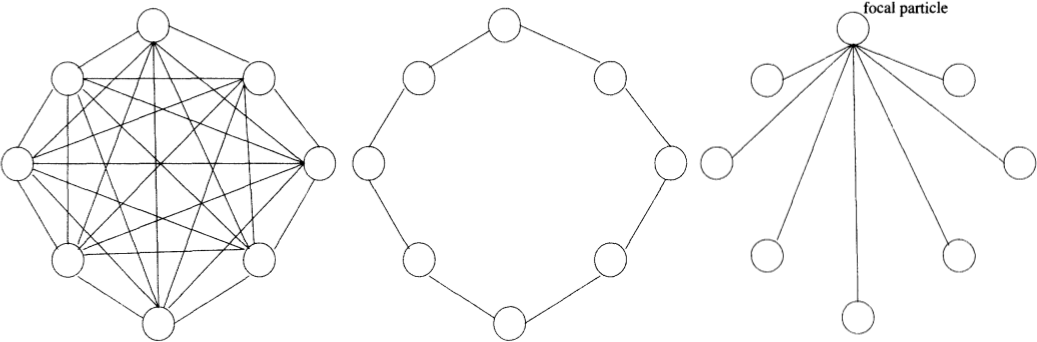
\includegraphics[width=\textwidth-\fboxrule-\fboxrule]{imgs/PSO.png}}
\end{figure}

\underline{Nota:} La vecidad se determina según \textbf{índices numéricos}, y no por medidas especiales (como la \textit{distancia euclídeana}, por ejemplo).

\subsubsection{Algoritmo}

Sea $\mathbf{x}_i(t)$ la posición de la partícula $P_i$ en el hiperspacio, en la iteración $t$. La posición de $P_i$ es modificada por la velocidad $\mathbf{v}_i(t)$ de acuerdo a:
\begin{equation}\label{eq:mov_pso}
\mathbf{x}_i(t) = \mathbf{x}_i(t-1)+\mathbf{v}_i(t).
\end{equation}
A partir de esto, veremos tres diferentes algoritmos para resolver el problema, que difieren entre sí en la forma en que intercambian información social.

\subsubsection*{\underline{Individidual Best (\textit{pbest}):}}

Versión básica del algoritmo, en que las partículas sólo utilizan sus propias experiencias.

\begin{enumerate}
\item Inicializar el enjambre de partículas con valores de posición aleatorios en el hiperespacio.
\item Evalúo la \textit{performance} $\mathcal{F}$ de cada partícula en su posición actual.
\item Realizo la comparación junto a la asignación:
\[
	\texttt{if } \left( \mathcal{F} (\mathbf{x}_i(t)) < \textit{pbest}_i \right) \texttt{ then: } \left\{
	\begin{array}{l}
	\textit{pbest}_i = \mathcal{F}(\mathbf{x}_i(t)),\\
	\mathbf{x}_{\textit{pbest}_i} = \mathbf{x}_i(t).
	\end{array}
	\right.
\]
\item Y luego cambiamos la velocidad cada partícula haciendo:
\[
\mathbf{v}_{i}(t) = \mathbf{v}_{i}(t-1) + \rho(\mathbf{x}_{\textit{pbest}_i}- \mathbf{x}_i(t)).
\]
dónde $\rho$ es un número positivo aleatorio.
\item Movemos a la partícula a la nueva posición (usando \ref{eq:mov_pso}) y avanzamos una iteración $t=t+1$.
\item Volver al paso (2), y repetir hasta \textit{convergencia}.
\end{enumerate}

A medida que más se aleja la partícula de su \textit{pbest}, mayores son los cambios en la velocidad para retornar a esa posición. El valor de $\rho$ influye en como la trayectoria de una partícula oscila. Mientras más chico $\rho$, más suave es la trayectoria.

\subsubsection*{\underline{{Global Best (\textit{gbest})}}}

Refleja la topología \textbf{estrella}. La experiencia de cada partícula es compartida hacia el resto, influyendo en los movimientos de estos.

El algoritmo es similar al \textit{pbest}, exceptuando el agregado un nuevo paso luego del (3), y el cambio en la fórmula de calcular la velocidad de la partícula:

\begin{enumerate}
\setcounter{enumi}{3}
\item Luego de realizar la comparación con la asignación, se procede a determinar el \textit{gbest}:
\[
	\texttt{if } \left( \mathcal{F} (\mathbf{x}_i(t)) < \textit{gbest} \right) \texttt{ then: } \left\{
	\begin{array}{l}
	\textit{gbest} = \mathcal{F}(\mathbf{x}_i(t)),\\
	\mathbf{x}_{\textit{gbest}} = \mathbf{x}_i(t).
	\end{array}
	\right.
\]
\item Y el cambio en la velocidad está dado por:
\begin{align*}
\mathbf{v}_{i}(t) &= \mathbf{v}_{i}(t-1) + \rho_1(\mathbf{x}_{\textit{pbest}_i}- \mathbf{x}_i(t)) + \rho_2(\mathbf{x}_{\textit{gbest}}- \mathbf{x}_i(t)),\\
&= \mathbf{v}_{i}(t-1) + \text{componente \textit{cognitiva}} + \text{componente \textit{social}}.
\end{align*}
dónde se ha incorporado el término de \textit{gbest}, siendo $\rho_1$, $\rho_2$, variables aleatorias.
\end{enumerate}

El resto del algoritmo procede igual que el de $pbest$. 

Mientras más alejado esté la partícula del \textit{gbest} y de su propio \textit{pbest}, el cambio en la velocidad para retornar a su mejor posición será mayor. Las variables $\rho_1$ y $\rho_2$ están definidas como $\rho_i=r_i\,c_i$, con $r_i \sim U(0,1)$, y $c_i$ una constante positiva de aceleración. Para evitar diverger, $c_1 + c_2 \leq 4$.

\subsubsection*{\underline{Local Best (\textit{lbest})}}

Refleja la topología \textbf{anillo}. Las partículas son sólo influenciadas por sus propios \textit{pbest}, como así también por la mejor posición de su vecino \textit{lbest}. Del algoritmo \textit{gbest} sólo cambia el paso (4) y (5) al reemplazar \textit{gbest} por \textit{lbest}.

A pesar de ser \textit{lbest} \textbf{más lento} en converger que \textit{gbest}, presenta mejores soluciones y busca en un área mucho más grande del espacio de búsqueda.

\subsubsection{Convergencia}

La convergencia se llega cuando el PSO cumple un cierto número de iteraciones, cuando su mejor \textit{performance} ha cruzado un umbral, o cuando los cambios en las velocidades de las partículas son cercanos a cero.

\subsubsection{Parámetros del Sistema}

\begin{enumerate}
\item \textbf{Dimensión del problema.} El PSO funciona mejor en problemas de altas dimensiones.
\item \textbf{Número de individuos.} Depende del problema en sí y la cantidad de dimensiones de este.
\item \textbf{Límite superior de $p$.} Depende del grado de oscilación en la trayectoria de las partículas buscado.
\item \textbf{Velocidad máxima $V_{\max}$.} Previene que las partículas abandonen rápidamente una región del espacio sin explorarla adecuadamente. Es usualmente proporcional al tamaño del problema.
\item \textbf{Tamaño de la vecindad.} Existe un compromiso entre la cantidad de vecinos (mayor área de búsqueda, menos posibilidad de caer en un mínimo local) y la rapidez de convergencia.
\item \textbf{Peso inercial.} Se puede mejorar la \textit{performance} del PSO a través de su incorporación en el cálculo de velocidad:
\[
\mathbf{v}_{i}(t) = \phi \, \mathbf{v}_{i}(t-1) + \text{componente \textit{cognitiva}} + \text{componente \textit{social}}.
\]
dónde $\phi$ es el \textbf{peso inercial}. Este controla la influencia de las velocidades anteriores en las nuevas velocidades. Es conveniente irlo modificando a través del tiempo, comenzando en un $\phi$ alto, para búsquedas en áreas más grandes, e irlo disminuyendo al valor para ir refinando la búsqueda en áreas más chicas.
\end{enumerate}

\underline{Nota:} para que la convergencia sea posible, debe darse que: $\phi > \frac{1}{2} (c_1 + c_2) - 1$.

\subsubsection{Comparación con los algoritmos genéticos}

\begin{itemize}
\item Ambos usan reglas de transición \textbf{probabilíticas}.
\item Ambos están  basados en adaptación, pero en el PSO los cambios son obtenidos a través del aprendizaje entre iguales, no entre operadores de variación.
\item El PSO tiene memoria: las partículas guardan registro de las mejores soluciones, y las velocidades anteriores son usadas para ajustar posiciones.
\item El PSO no tiene función de \textit{fitness}: el proceso de búsqueda es guíado por interacciones sociales entre partículas.
\end{itemize}

\subsection{Colonias de Hormigas}

\subsubsection{Inspiración biológica}

En las colonias de hormigas, la distribución y ejecución de las tareas está basada en diferencias anatómicas en los individuos (\textit{que distinguen hormigas obreras de soldados, por ejemplo}) y en la \textbf{estigmergía}.

Se observan \textbf{conductas emergentes} cuando los agentes individuales prestan atención a sus vecinos inmediatos sin esperar órdenes, y actúan localmente. La acción colectiva de estos agentes produce el comportamiento global. Dentro de una colonia de hormigas, las mismas piensan localmente y  actúan localmente, pero producen comportamiento global.

La \textbf{estigmergía} hace referencia al comportamiento distribuído dentro de la colonia de hormigas, siendo caracterizada por:
\begin{itemize}
\item La falta de una coordinación centralizada.
\item La comunicación y la coordinación entre los individuos se basa en modificaciones locales del ambiente.
\item Retroalimentación positiva, que refuerza las acciones (\textit{por ejemplo, las feromonas para seguir rastros de comida}).
\end{itemize}

La \textbf{estigmergía artificial} está definida como la comunicación indirecta mediada por modificaciones numéricas de los estados ambientales que son solos localmente accesibles por los agentes comunicadores. La esencia de modelar colonias de hormigas es el encontrar un modelo matemático que describa de forma precisa las características de \textbf{estigmergía} (``\textit{invisible manager}'') correspondientes a cada individuo.

\subsubsection{Feromonas}

Las hormigas tienen la habilidad de siempre encontrar el \textbf{camino más corto} entre su nido y la fuente de alimento. Este comportamiento puede ser explicado por las feromonas arrojadas por cada hormiga. Durante la búsqueda por comida, y al regresar de la fuente de comida al nido, cada hormiga libera feromonas que se depositan en el camino. Para elegir un camino a seguir, las hormigas siguen el camino con mayor concentración de feromonas. El camino \textbf{más corto} va a tener un depósito de feromonas mucho más fuerte que el camino más largo, dado a que el \textbf{retorno} por ese camino desde la fuente de alimentos es \textbf{más rápido} (\textit{nótese que liberan más feromonas de regreso al nido con alimento}). Además, el depósito de feromonas \textbf{se evapora con el tiempo}, por lo que la fuerza del depósito de feromonas se va decrementar mucho más rápido en el camino más largo que en el corto.

\subsubsection{Algoritmo básico}

\begin{enumerate}
\item Comportamiento inicial aleatorio.
\item Cuando encuentran una fuente de comida, se organizan y comienzan a seguir el nuevo camino.
\begin{enumerate}[2.1]
\item Mecanismo de reclutamiento: mayormente por \textbf{feromonas}, liberados al regresar.
\item Si otros encuentran el rastro, lo seguirán probablemente.
\item El rastro se refuerza al ser seguido por más hormigas (pero se va evaporando).
\end{enumerate}
\end{enumerate}

\section{Lo que le tomaron a Marcus}
SOM, logica difusa, y enjambre de particulas y q les cuente como funcionaba. El teorema de la entropia borrosa eso fue lo mas especifico q me preguntaron

\end{document}
